\documentclass[tikz,border=2pt]{standalone}

\usepackage{pgfplots}
\usetikzlibrary{positioning}
\usepgfplotslibrary{}
\pgfplotsset{compat=1.18,width=4.5cm,height=6cm}


\begin{document}
	
	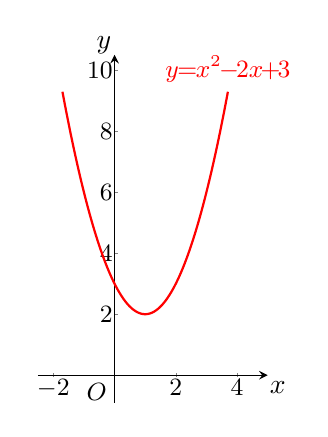
\begin{tikzpicture}
		\begin{axis}[
			clip=false,
			axis lines=center,
			no markers,
			xmin=-2.5,xmax=5,
			ymax=10.5,ymin=-0.9,		
%			xticklabels={0.2,0.4,0.6},
			xtick={-2,2,4},
%			xtick distance=1,
%			ytick distance=1,
			ytick={2,4,6,8,10},
			yticklabels={2,4,6,8,10},
			yticklabel style={font=\small\rmfamily},
			xticklabel style={font=\small\rmfamily},
			ytick align=inside,
			major tick length=0.5mm, 
			yticklabel shift=-1mm,
			xticklabel shift=-1mm,
			ylabel=$y$,xlabel=$x$,
			xlabel shift=-1em,
			ylabel shift=1cm,
			xlabel style={xshift=1em,yshift=-1em},
			ylabel style={xshift=-1em,yshift=1em},
			]
			\addplot+ [samples=100,domain=-1.7:3.7,red,thick,]{x^2-2*x+3};
			\addplot[samples at={3.7}]{x^2-2*x+3}node[above,red]{\small $y\!\!=\!\!x^2\!\!-\!\!2x\!\!+\!\!3$};
			\node at(0,0) [below left=-1pt]{\small $O$};
            \end{axis}           
	\end{tikzpicture}
	
\end{document}